\documentclass[11pt,a4paper]{article}

\usepackage[margin=2.5cm]{geometry}
\usepackage[T1]{fontenc}
\usepackage{lmodern}
\usepackage{microtype}
\usepackage{graphicx}
\usepackage{booktabs}
\usepackage{float}
\usepackage{amsmath}
\usepackage{hyperref}

\title{Task 2: Location Clusters in NYC Taxi Pickups}
\author{}
\date{}

\begin{document}
\maketitle

\section{Location Clusters}
\label{sec:location-clusters}

Taxi demand in New York is concentrated in space and shifts through the day and week. This section maps that concentration with pickup heatmaps (Section~\ref{sec:heatmaps}) and then locates individual hotspots with DBSCAN for two driver-relevant periods (Section~\ref{sec:dbscan}).

All analysis uses the cleaned trips (1,442,031 of 1,458,644 records, 98.86\% retained after removing implausible durations, speeds, distances, passenger counts and coordinates). Pickups are further restricted to the map window
\[
-74.05 \leq \text{longitude} \leq -73.75,\qquad
40.63 \leq \text{latitude} \leq 40.85,
\]
which covers Manhattan, the western edge of Queens, northern and western Brooklyn, and both major airports.

%--------------------------------------------------------------------
\subsection{Heatmaps}
\label{sec:heatmaps}

\subsubsection{Choice of morning and evening bands}

With roughly 1.4 million trips, a scatter plot saturates into a solid blob, so pickups are binned into grid cells and the cell counts are drawn as a heatmap. Trips are split by day type (Monday--Friday against Saturday--Sunday) and by time of day. The time bands come from the hourly pickup profile in Figure~\ref{fig:hourly}.

\begin{figure}[H]
\centering
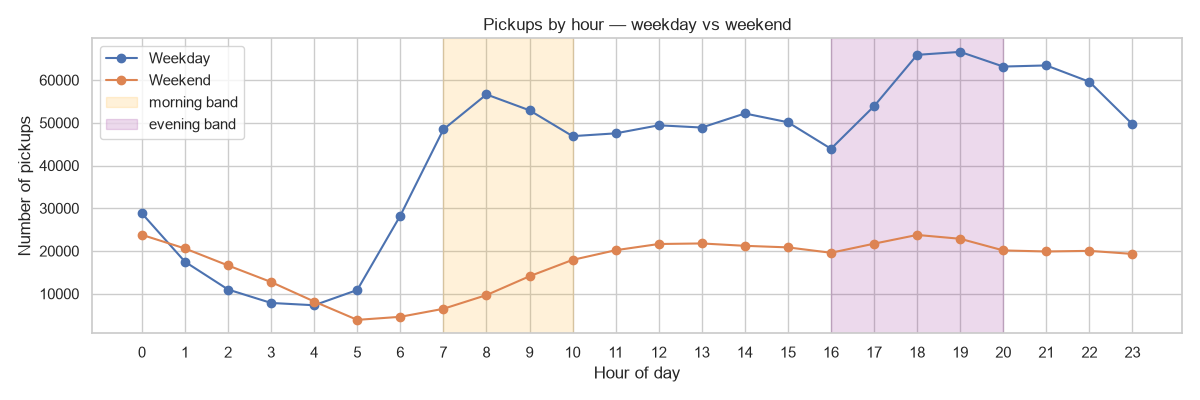
\includegraphics[width=\textwidth]{pickups_in_a_day.png}
\caption{Total pickups by hour of day for weekdays and weekends. The shaded areas mark the morning band (07:00--09:59) and the evening band (17:00--19:59).}
\label{fig:hourly}
\end{figure}

The weekday profile has two clear features:
\begin{itemize}
    \item \textbf{Morning peak.} Pickups climb from about 11,000 at 05:00 to about 57,000 at 08:00, then drop to about 47,000 by 10:00 and stay between roughly 47,000 and 52,000 through the afternoon. The 08:00 maximum is the only pre-noon peak, so 07:00--09:59 captures the rise (07:00, about 48,000), the peak and the decline (09:00, about 53,000). A wider band starting at 06:00 would add an hour at about 28,000 that belongs to the ramp-up rather than the peak; a one-hour band at 08:00 would discard the shoulders that carry most of the volume.
    \item \textbf{Evening peak.} Pickups rise from a trough of about 44,000 at 16:00 to about 66,000 at 18:00 and 19:00, the highest values of the day. Demand stays elevated into the night (about 63,000 at 20:00 and 21:00, 60,000 at 22:00), so the evening is a broad plateau and not a narrow spike. The band 17:00--19:59 covers the steep rise and the two peak hours while staying clear of the late-evening hours, where the mix shifts towards leisure trips. This is the same window used in the second analysis for Thursday evening (17:00--20:00), which keeps the two parts of the section comparable.
\end{itemize}

Weekend volumes are much lower per hour and have no commute peak. Pickups are lowest at 05:00 (about 4,000), rise gradually through the morning, and sit between about 20,000 and 24,000 from 11:00 onwards, peaking weakly at 18:00. Weekend nights are comparatively busy: the 00:00 hour (about 24,000) exceeds the weekend morning band.

The same hours are used for both day types so that day type is the only variable that changes between panels. A weekend ``morning'' therefore is not a commute window; it measures where people are picked up in the same clock hours when commuters dominate on weekdays. The weekday--weekend gap in Figure~\ref{fig:hourly} must also be read against the number of days: weekdays are five days and weekends two, so raw totals are not per-day rates. Daily volume is in fact almost identical across the week (mean of 206,000 pickups per weekday against 206,000 per weekend day, from the day-of-week counts of the cleaned data), so the difference in hourly totals reflects the 5:2 day ratio plus a change in timing.

The timing change is visible in the share of each day type's pickups that fall in each band:
\begin{table}[H]
\centering
\caption{Pickups per group and share of all pickups on that day type (approximate; shares use day-of-week totals of the cleaned data).}
\begin{tabular}{lrrrr}
\toprule
 & \multicolumn{2}{c}{Weekday} & \multicolumn{2}{c}{Weekend} \\
\cmidrule(lr){2-3}\cmidrule(lr){4-5}
Band & Pickups & Share & Pickups & Share \\
\midrule
Morning (07:00--09:59) & 157,911 & 15.3\% & 30,203 & 7.3\% \\
Evening (17:00--19:59) & 186,291 & 18.1\% & 68,272 & 16.6\% \\
\bottomrule
\end{tabular}
\label{tab:groups}
\end{table}
The morning band holds twice as large a share of weekday trips as of weekend trips, while the evening band holds a similar share on both day types. Weekday mornings are therefore the most distinctive of the four groups, and the weekday and weekend evenings the most alike.

\subsubsection{Grid construction}

Each group's pickups are counted on one regular grid and every cell count is divided by the group's total, so each cell is the share of that group's pickups. This is needed because the groups differ in size by a factor of six (30,203 to 186,291 pickups); raw counts would make weekday groups look brighter everywhere without saying anything about where trips occur. All four panels share one logarithmic colour scale, since cell shares span about three orders of magnitude (from below $10^{-5}$ to above $10^{-2}$) and a linear scale would show only Midtown.

Two grid versions are shown. The first (Figure~\ref{fig:heatmap-grid}) uses 150 bins in longitude and latitude, about 169\,m by 163\,m per cell, drawn on plain coordinates with the full range of cell shares on the colour scale. The cell size is close to the 150\,m clustering radius used in Section~\ref{sec:dbscan}, so the heatmaps and the hotspot analysis resolve the city at a similar scale. The second (Figure~\ref{fig:heatmap-street}) uses a coarser 100-by-100 grid in Web Mercator coordinates (about 250\,m cells) over an OpenStreetMap background, so cells can be matched to streets and neighbourhoods. Its colour scale runs from the 5th to the 99.5th percentile of non-empty cell shares, which prevents the few extreme cells (Midtown and the airports) from compressing the rest of the range; cells above the upper limit are drawn at maximum brightness.

\begin{figure}[H]
\centering
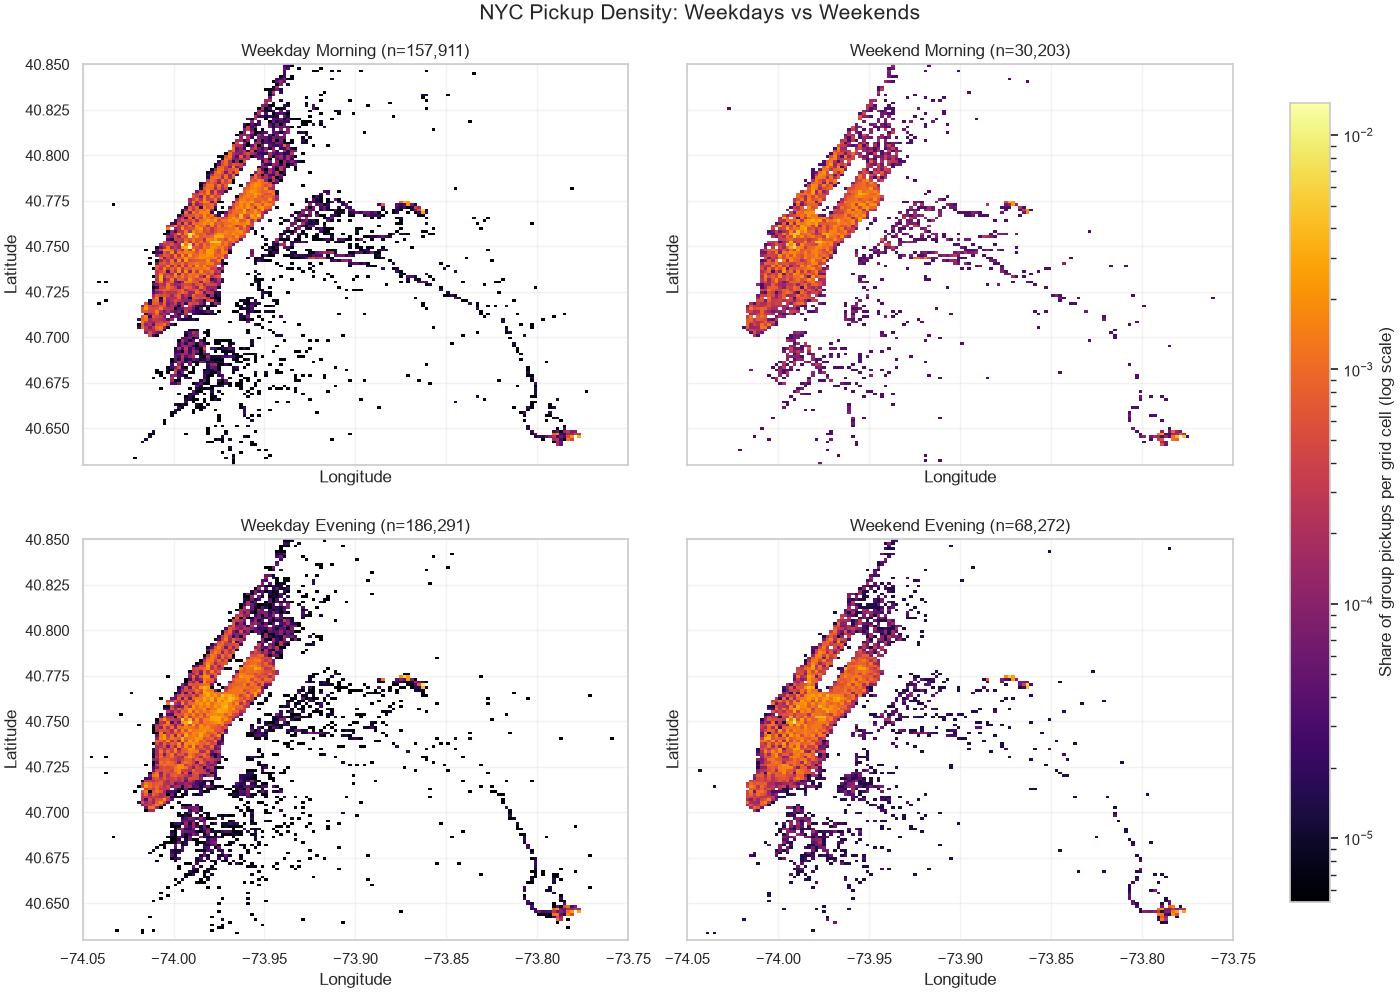
\includegraphics[width=\textwidth]{nyc_pickup_hitmap.png}
\caption{Pickup density for weekday and weekend mornings and evenings on a 150-by-150 grid (about 165\,m cells). Cell values are the share of each group's pickups; the colour scale is logarithmic and common to all panels.}
\label{fig:heatmap-grid}
\end{figure}

\begin{figure}[H]
\centering
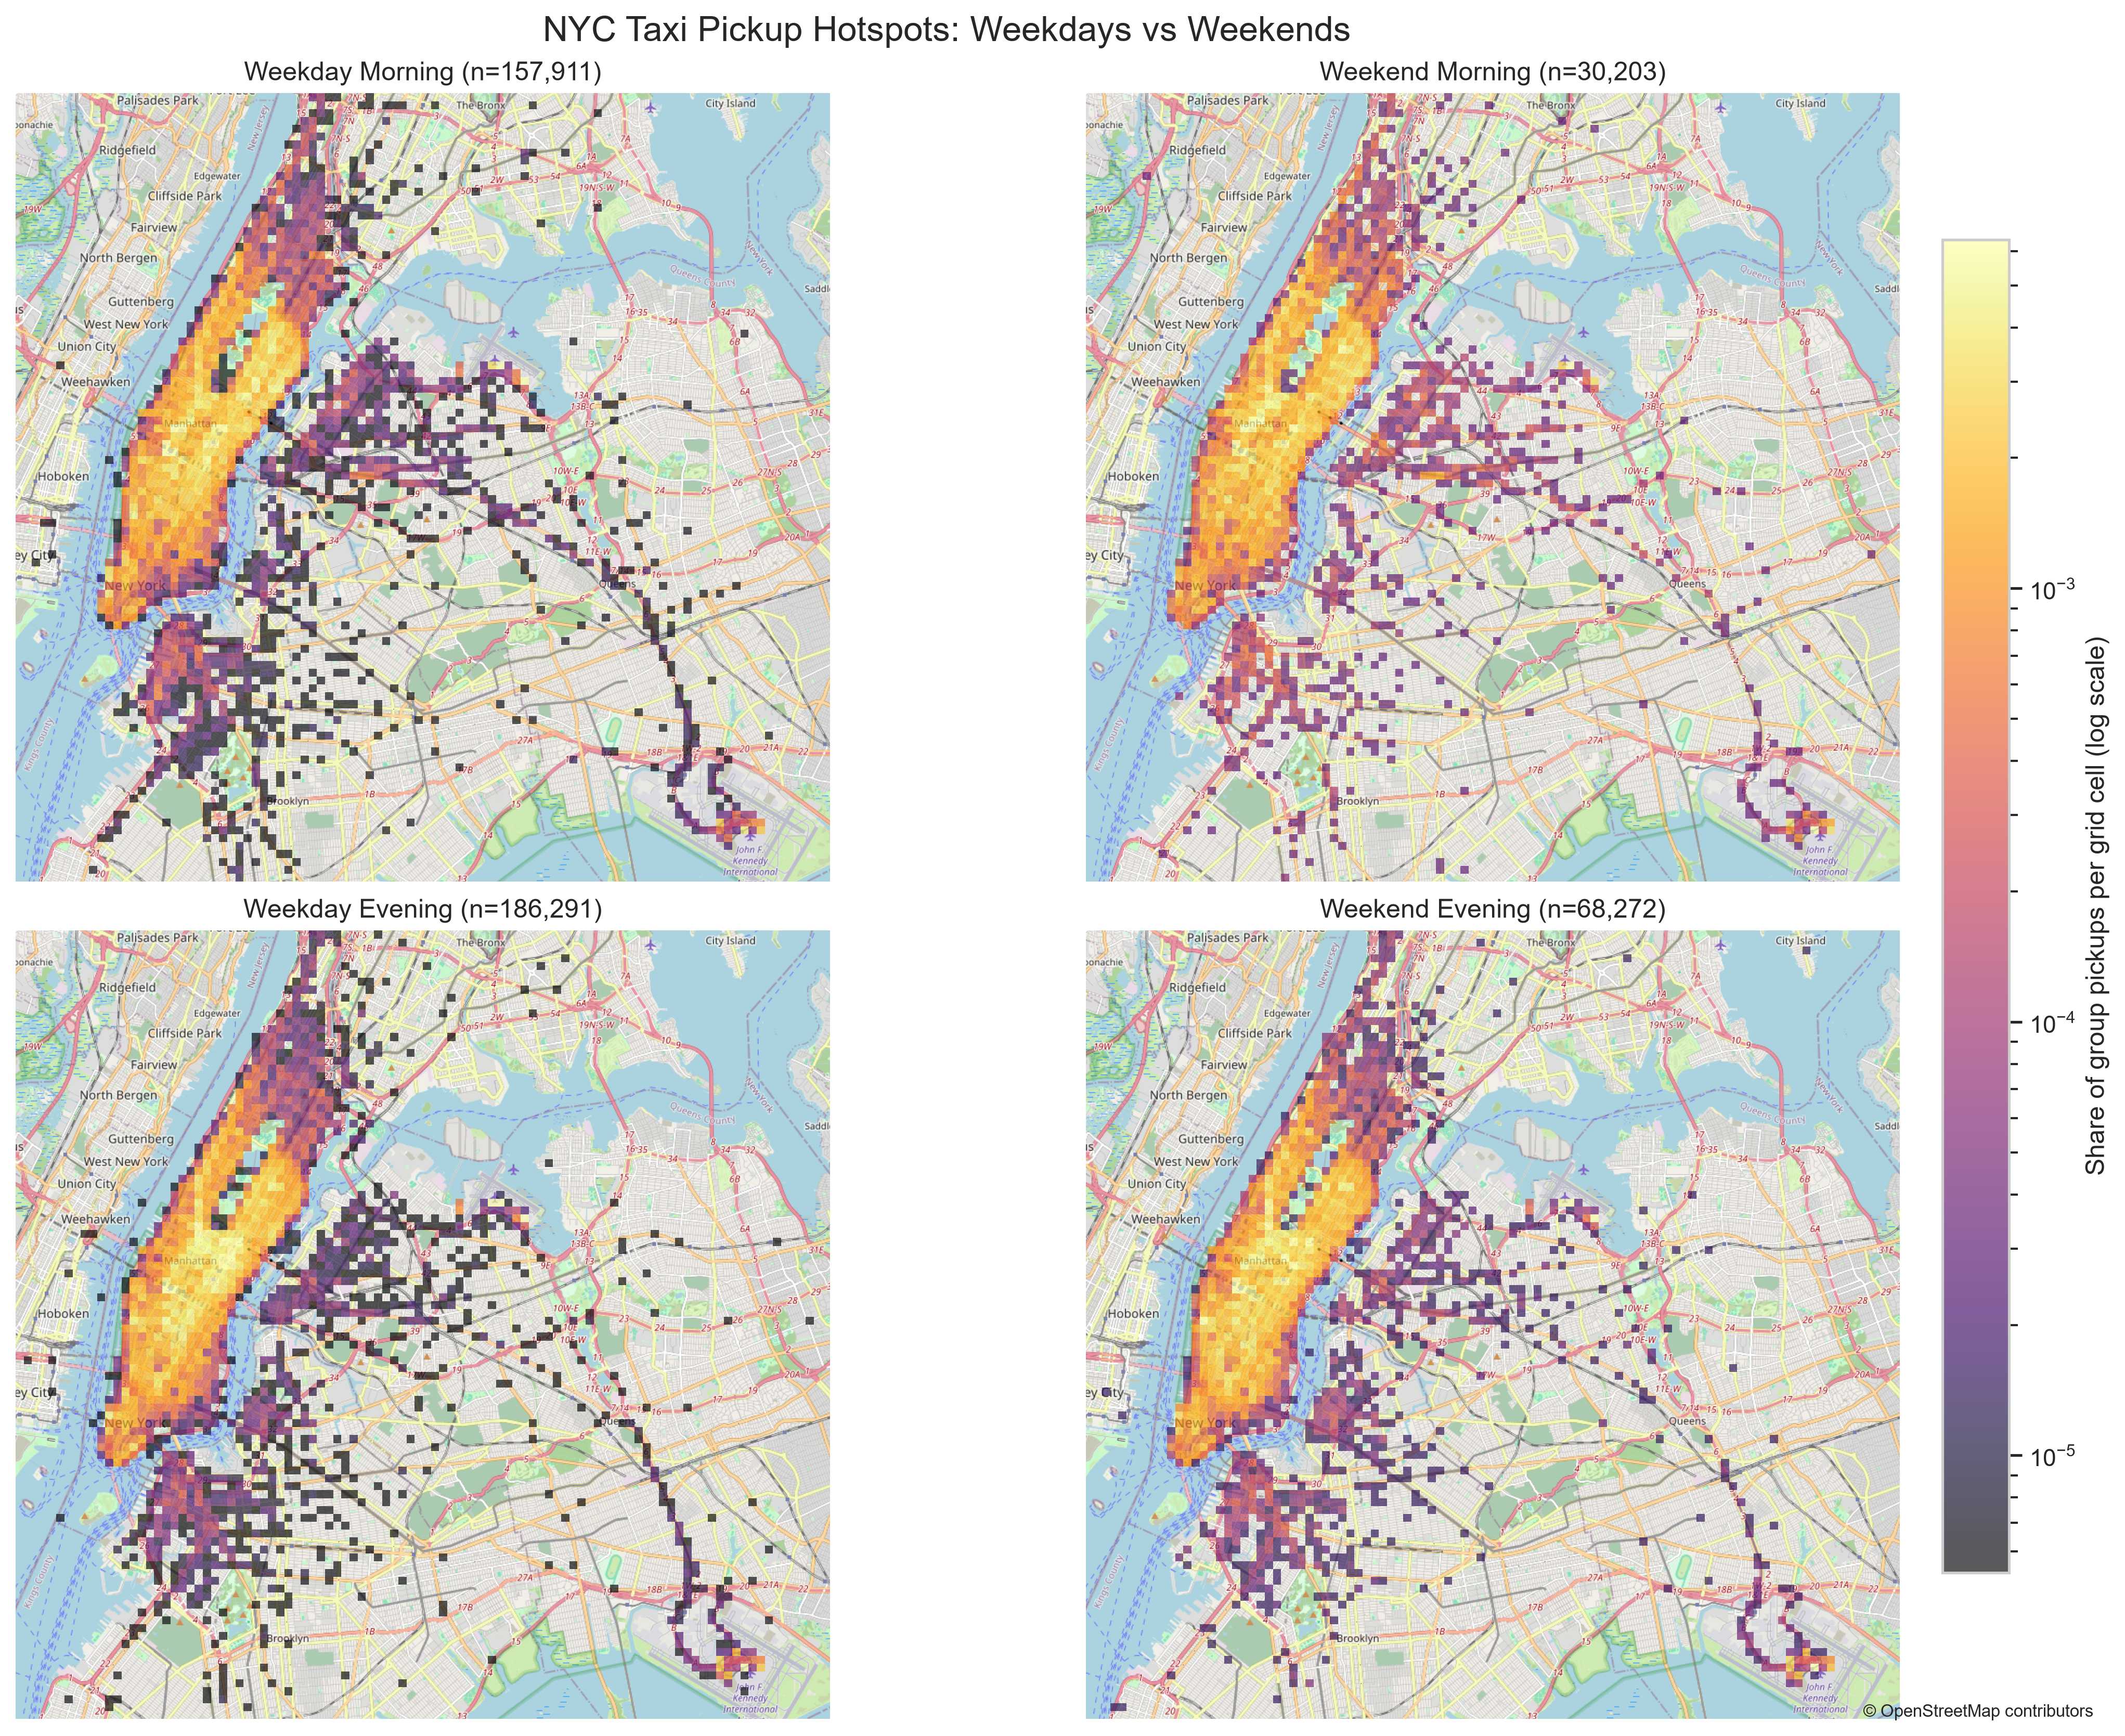
\includegraphics[width=\textwidth]{nyc_static_pickup_heatmaps.png}
\caption{The same four groups on a 100-by-100 grid (about 250\,m cells) over a street map, with a common logarithmic colour scale clipped at the 5th and 99.5th percentiles. Map tiles: \copyright\ OpenStreetMap contributors.}
\label{fig:heatmap-street}
\end{figure}

\subsubsection{Findings}

\begin{itemize}
    \item \textbf{Demand is concentrated in Manhattan in every group.} The brightest cells form a band from the Financial District to roughly Harlem, strongest in Midtown and the Midtown-south corridor. Central Park appears as a dark hole in the middle of the band because there are few pickup points inside it. Outside Manhattan, pickups are sparse and form isolated cells.
    \item \textbf{The airports are the only bright cells outside Manhattan.} LaGuardia (about $-73.87$, $40.77$) and JFK (about $-73.78$, $40.65$) are visible in all four panels, and a thin trail of cells along the expressways linking JFK and LaGuardia to Manhattan is also visible. Airport pickups are the one non-Manhattan source of concentrated demand at every time studied.
    \item \textbf{Weekday mornings spread further into the outer boroughs.} The weekday morning panel shows the strongest secondary concentrations in downtown Brooklyn and in western Queens across the East River, consistent with commuters from residential areas heading into Manhattan. These areas are present but weaker on weekend mornings, where activity is dominated by Manhattan.
    \item \textbf{Evenings look similar across day types.} The weekday and weekend evening panels have a nearly identical Manhattan core, in line with the similar evening shares in Table~\ref{tab:groups}. The weekend evening panel shows more cells in north-west Brooklyn, in the Williamsburg--Greenpoint direction, than the weekday evening panel.
    \item \textbf{Sample size matters for the sparse areas.} Scattered single cells in the weekend morning panel (30,203 pickups) are partly a sample-size effect: a cell with one pickup there has a larger share than a cell with one pickup in the 186,291-pickup weekday evening panel, so the weekend panels look more speckled even where the underlying distribution is similar. Differences in the Manhattan core are reliable; differences between individual outer cells are not.
\end{itemize}

Because every cell is a share within its group, the maps show where trips start relative to the rest of that group, not how many trips there are. They show that concentration exists and where, but not why a given area has more pickups.

%--------------------------------------------------------------------
\subsection{Hotspot detection with DBSCAN}
\label{sec:dbscan}

\subsubsection{Periods and data}

A driver planning an evening wants the places with the most pickups in a given hour. Two periods are examined:
\begin{itemize}
    \item \textbf{Friday night:} Friday 23:00 to Saturday 02:00 (Friday 23:00--23:59 and Saturday 00:00--01:59).
    \item \textbf{Thursday evening:} Thursday 17:00 to 20:00 (17:00--19:59).
\end{itemize}
Pickups with missing timestamps or coordinates are dropped and the map window is applied. This leaves 34,868 pickups for Friday night and 38,255 for Thursday evening.

\begin{table}[H]
\centering
\caption{Pickup records selected for DBSCAN.}
\begin{tabular}{lrr}
\toprule
Period & Selected pickups & Hourly windows (26 weeks) \\
\midrule
Friday night (23:00--02:00) & 34,868 & 78 \\
Thursday evening (17:00--20:00) & 38,255 & 78 \\
\midrule
Total & 73,123 & 156 \\
\bottomrule
\end{tabular}
\end{table}

Each period spans three hours a week over the 26 weeks of the data, giving 78 separate hour-long windows per period and 156 in total. This corresponds to about 450 pickups per Friday-night hour and about 490 per Thursday-evening hour across the whole map window.

\subsubsection{Method and parameter choice}

DBSCAN is used because the number of hotspots is not known beforehand. It grows clusters from points that have enough neighbours within a radius $\varepsilon$ and labels isolated points as noise, so it needs no preset cluster count and does not force every pickup into a cluster, unlike k-means. Distances are great-circle (haversine) distances on coordinates converted to radians in latitude--longitude order, so $\varepsilon$ is a true ground distance rather than a distance in degrees. Each hour-long window is clustered separately, since a hotspot is defined as a location with many pickups \emph{within one hour}; pooling hours would merge places that are busy at different times with places that are busy at the same time.

\paragraph{Minimum samples.} A hotspot requires at least 15 pickups within the neighbourhood in an hour, so \texttt{min\_samples} $=15$. This is one pickup every four minutes at a single location. It is a demanding threshold: a circle of radius 150\,m has an area of 0.07\,km$^2$, and 15 pickups represent about 3\% of the roughly 450--490 pickups the entire map window produces in an average hour of these periods.

\paragraph{Radius.} The radius is
\[
\varepsilon = \frac{0.15}{6371.0088}\ \text{radians}\ (= 150\ \text{m}),
\]
where 6371.0088\,km is the mean Earth radius. A radius of 150\,m was chosen over the 50--100\,m range because:
\begin{itemize}
    \item Manhattan blocks are about 80\,m between cross streets and 250--280\,m between avenues, so 50\,m cannot span even one block face; 150\,m covers a street corner and its adjoining frontage, which is the area a driver can serve from one position.
    \item Urban-canyon GPS error between tall buildings is commonly tens of metres, so a very small radius splits one pickup spot into several fragments.
    \item The threshold is already strict. The detected clusters contain 15 to 17 pickups, meaning they only just exceed \texttt{min\_samples}. Reducing $\varepsilon$ reduces the number of neighbours each point can have, so smaller radii would find fewer, or no, clusters under the same threshold.
\end{itemize}
The cost of 150\,m is a coarser location: a cluster centre can lie up to one block from the exact origin of its pickups. The results are conditional on this radius, and because the clusters sit at the minimum size, a change in either parameter would change the count. A comparison across several radii and thresholds would quantify that sensitivity; it has not been run here.

For each cluster the mean latitude, mean longitude and pickup count are recorded. Noise points are excluded.

\subsubsection{Results}

Six clusters are detected among the 156 hourly windows: four in Friday-night windows and two in Thursday-evening windows. Most windows (96\%) contain no cluster at all, so a pickup concentration meeting the threshold is rare.

\begin{table}[H]
\centering
\caption{Hourly DBSCAN cluster detections with approximate locations.}
\label{tab:clusters}
\footnotesize
\begin{tabular}{llrrrl}
\toprule
Period & Hour beginning & Latitude & Longitude & Pickups & Approximate area \\
\midrule
Thursday evening & 2016-01-28 19:00 & 40.770 & $-73.863$ & 17 & LaGuardia Airport \\
Friday night & 2016-01-30 01:00 & 40.719 & $-73.990$ & 16 & Lower East Side \\
Friday night & 2016-03-26 01:00 & 40.723 & $-73.987$ & 16 & East Village \\
Friday night & 2016-04-16 01:00 & 40.740 & $-74.006$ & 16 & West Village \\
Friday night & 2016-06-11 01:00 & 40.741 & $-74.006$ & 15 & West Village \\
Thursday evening & 2016-01-07 18:00 & 40.749 & $-73.992$ & 15 & Midtown (Penn Station area) \\
\bottomrule
\end{tabular}
\end{table}

\begin{figure}[H]
\centering
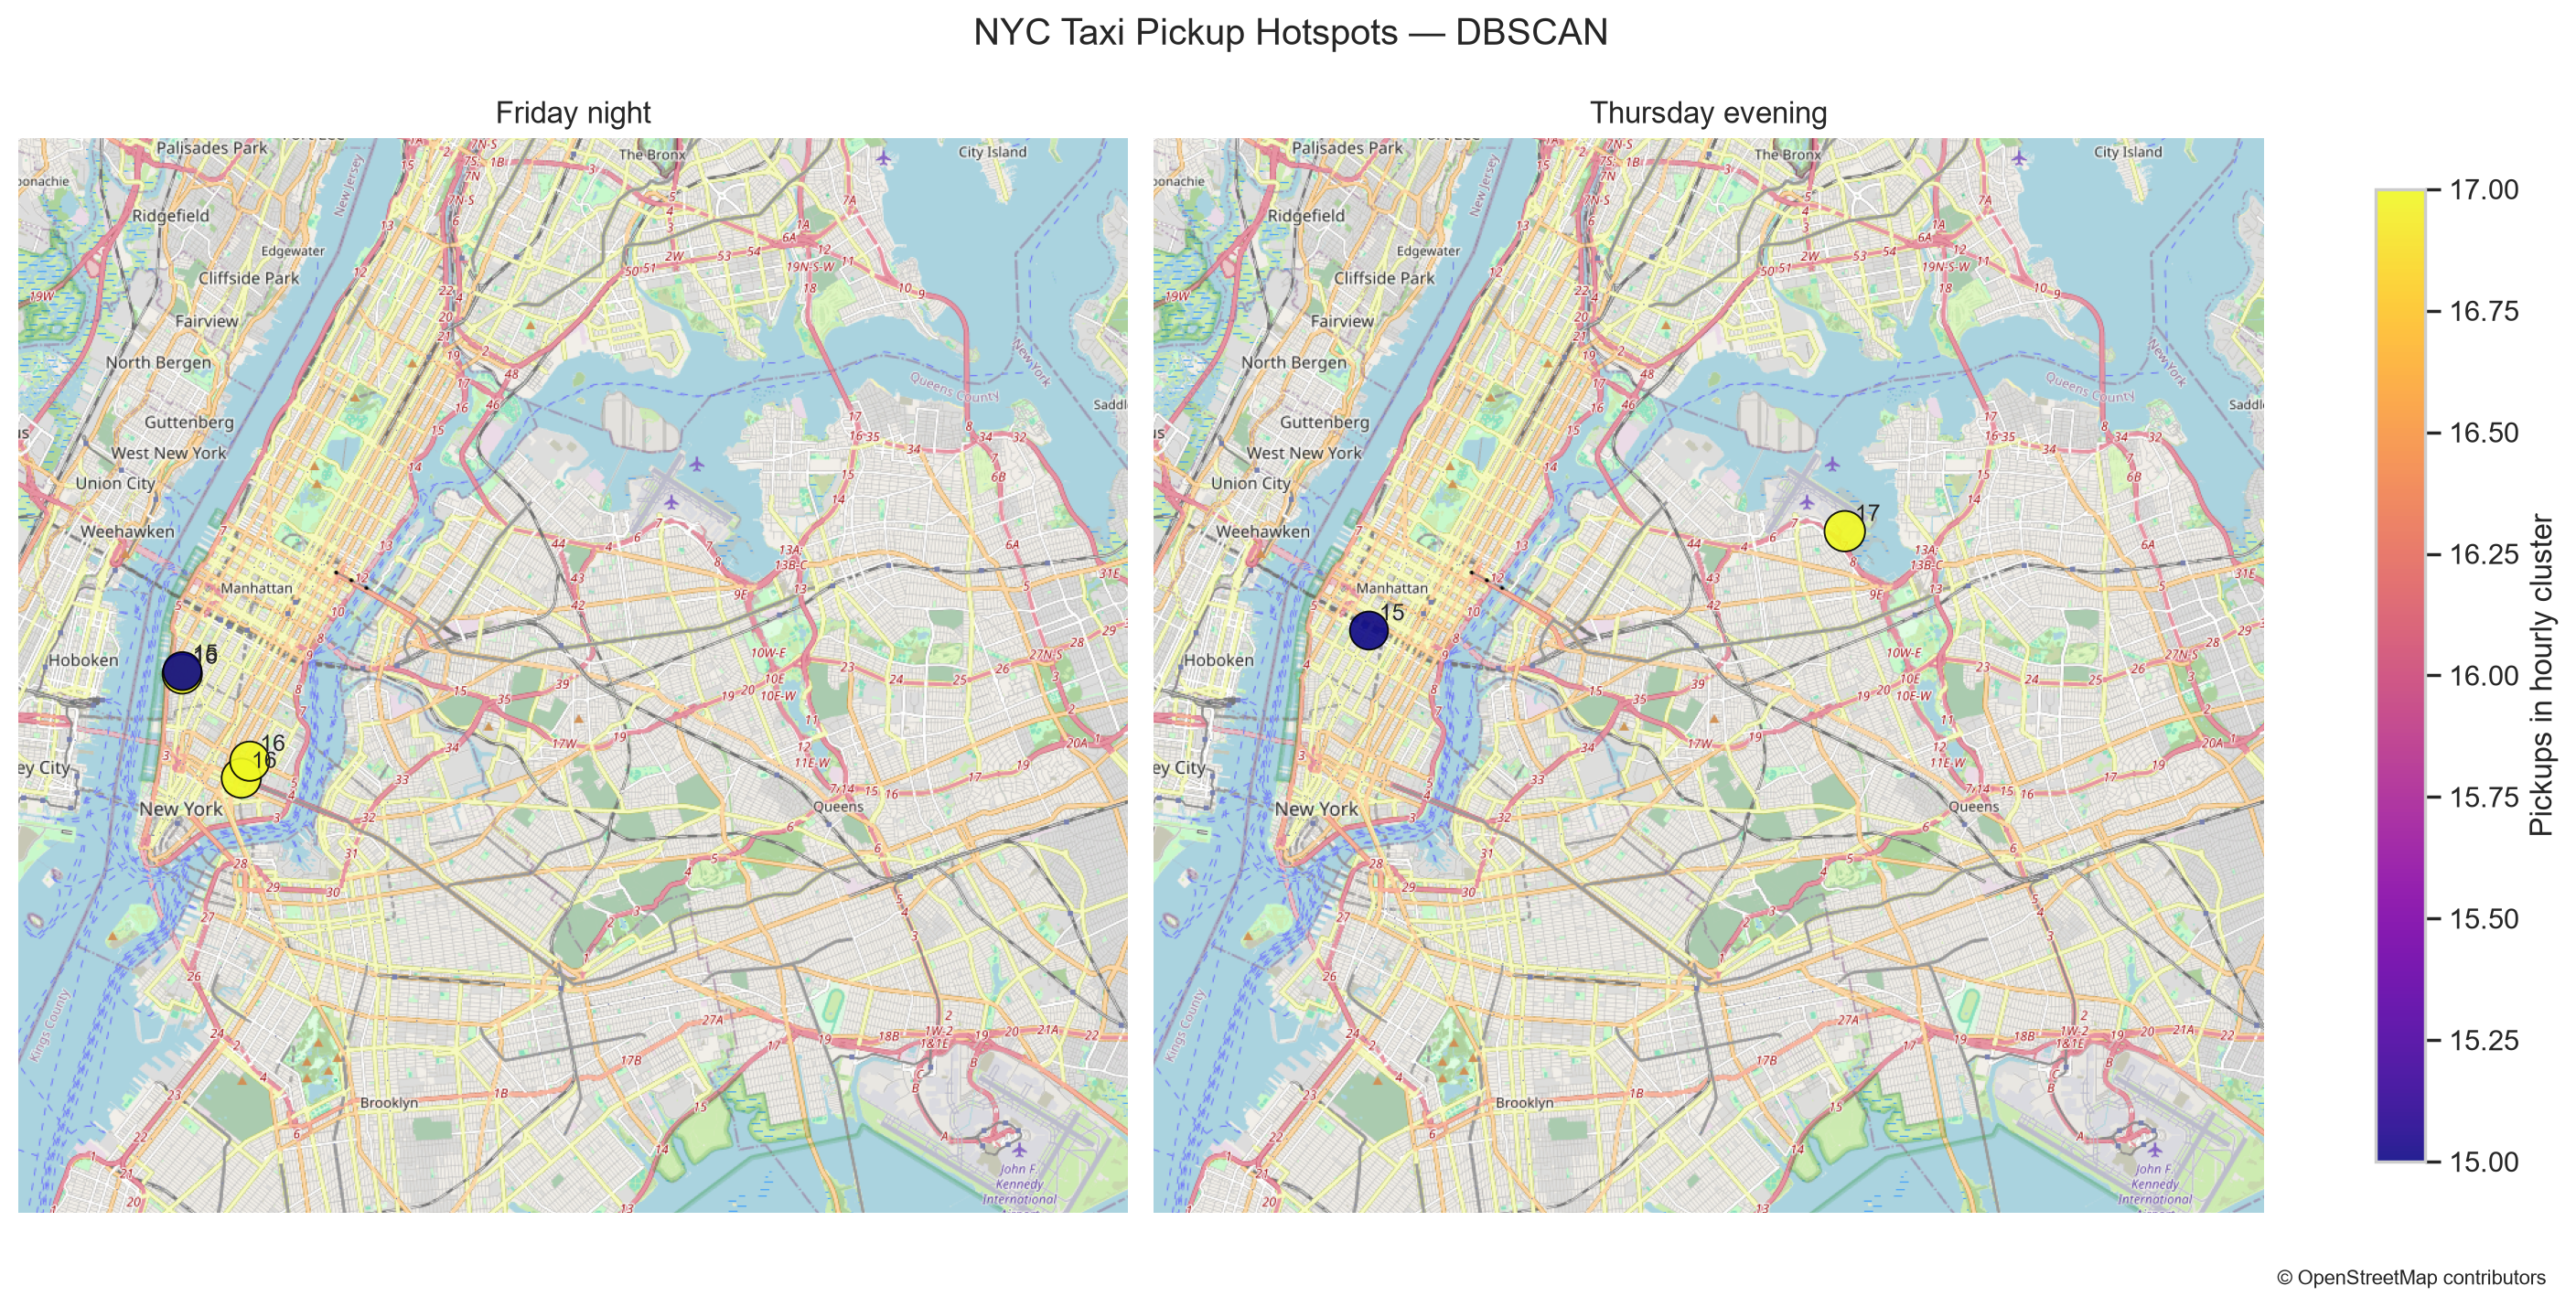
\includegraphics[width=\textwidth]{nyc_dbscan_street_map.png}
\caption{Hourly DBSCAN cluster centres for Friday night (left) and Thursday evening (right). Marker size and colour give the number of pickups in the cluster. Map tiles: \copyright\ OpenStreetMap contributors.}
\label{fig:dbscan-map}
\end{figure}

Three patterns stand out:
\begin{itemize}
    \item \textbf{Friday-night hotspots are nightlife areas at closing time.} All four Friday-night clusters fall in the 01:00--01:59 hour on a Saturday, and all lie in the downtown nightlife districts of the Lower East Side, East Village and West Village. None appears in the 23:00 or 00:00 hours, when pickups are spread more widely.
    \item \textbf{One location recurs.} Two Friday-night detections (16 and 15 pickups, April and June) are within about 100\,m of each other near $(40.74, -74.006)$ and overlap on the map, so the six detections represent five distinct locations. This repetition on different dates suggests the West Village is a repeatable late-night hotspot, though two observations are too few to establish a pattern.
    \item \textbf{Thursday evening hotspots are transport hubs.} The largest cluster (17 pickups, 19:00 on 28 January) is at LaGuardia Airport, consistent with the airport cells in the heatmaps, and the other is in Midtown near Penn Station.
\end{itemize}

\paragraph{Answer.} \textbf{Six} hourly clusters are found: four on Friday night and two on Thursday evening, covering five distinct locations. The result is small because the criterion is strict (15 pickups within 150\,m in a single hour) and because the data are not dense enough to meet it outside a handful of places and times. Every cluster is within two pickups of the minimum, so the exact number depends on the parameters. The heatmaps show where pickups are generally concentrated, which is a wider region than the places that reach this hourly threshold.

%--------------------------------------------------------------------
\subsection{Summary}

Weekday pickups peak at 08:00 and 18:00--19:00, and the bands 07:00--09:59 and 17:00--19:59 capture those peaks. Normalising each group's grid by its own total shows that Manhattan dominates at all times, that LaGuardia and JFK are the only strong concentrations outside it, and that weekday mornings reach furthest into Brooklyn and Queens. The weekday morning band holds about twice the share of the day's trips (15.3\%) that the weekend morning band does (7.3\%), while the evening bands are similar (18.1\% and 16.6\%).

DBSCAN with a 150\,m radius and 15-pickup minimum finds six hourly hotspots among 156 windows: four downtown nightlife clusters during the 01:00 hour after Friday night, and two on Thursday evening at LaGuardia and in Midtown. These findings depend on the map window, time bands and the radius and threshold; the clusters are at the lower limit of what the criterion allows.

\end{document}